\documentclass[12pt]{article}

% Packages
\usepackage[utf8]{inputenc} % allow utf-8 input
\usepackage[T1]{fontenc}    % use 8-bit T1 fonts
\usepackage{geometry}       % to change the page dimensions
\usepackage{graphicx}       % support the \includegraphics command and options
\usepackage{amsmath}        % for better mathematical formulas
\usepackage{amsfonts}       % for mathematical fonts
\usepackage{amssymb}        % for mathematical symbols
\usepackage{hyperref}       % for hyperlinks
\usepackage{lipsum}         % for generating filler text
\usepackage{float}          % for better figure placement
\usepackage{natbib}         % for better citations
\usepackage{pdfpages}
\usepackage{algorithm}
\usepackage{algpseudocode}
\usepackage{algorithmicx}       % for including pdfs
\bibliographystyle{unsrtnat}

% Page geometry
\geometry{a4paper, margin=1in}

\begin{document}

%Title Page
\begin{titlepage}
    \centering
    \vspace*{5cm}

    \Large
    \textbf{Multi-Agent SLAM: Exploration and Mapping in Simulated testing Environments}

    \vspace{1cm}

    Charlie Anthony [CandNo: 246537]\\
    Supervisor: Dr Chris Johnson



    \vfill

    \vspace{1cm}

    \small
    Dissertation\\
    Computer Science and Artificial Intelligence BSc

    
\includegraphics[width=0.3\linewidth]{sussex_logo.jpg}


    \small
    Department of Informatics and Engineering\\
    University of Sussex\\
    May 2024
\end{titlepage}

%Table of Contents
\tableofcontents
\newpage

\section{Introduction}
Swarms exist everywhere in life. Nearly all organisms exhibit some form of swarming behaviours within their
communities. Starlings display impressive organisational behaviour, positioning themselves with respect to the
movement of their neighbours. Humans show swarm behaviours when moving in crowds, for example, moving around sports
venues or exiting buildings in emergencies. No matter how hard you look, regardless if the context, swarms are
typically present.\\
These behaviours can also be artificially created in robotics. Within the realm of computing, parallelising
processes is breaking barrier after barrier - swarm robotics brings the same benefits. Being able to divide and
conquer a problem has the ability to massively increase the rate of work by employing multiple robots. Therefore, it
would be wasteful not to properly dedicate the time which this discipline deserves.\\
For my project, I am going to try and reproduce some of these behaviours artificially. I will start by simulating robotic
agents in a 2D environment. The agents will be placed within close proximity inside a simulated environment and then allowed
to explore and combine their findings; ultimately creating a visualization map of its environment. The agents will need to
both navigate the environment and avoid collisions, whilst creating an internal representation of its surroundings. The
best-case scenario for the agents within the swarm is to be fully independent; creating a decentralized system.\\
I will initially explore this problem by creating SLAM simulations, and then attempting to apply similar techniques
to a centralised system. These initial simulations will employ techniques such as graph-based SLAM, random walks and other elements of
swarm behaviours in order to create a base-line representation of the environment. This project will also have the flexibility to
potentially implement physical robots, given time permits.\\

%Professional and Ethical Considerations

%insert new page
\newpage

\section{Literature Review} % 3000 words - currently 2800

\subsection{Introduction to SLAM} % 300 words - currently 331

\begin{figure}[h]
    \centering
    \begin{minipage}{0.45\textwidth}
        \centering
        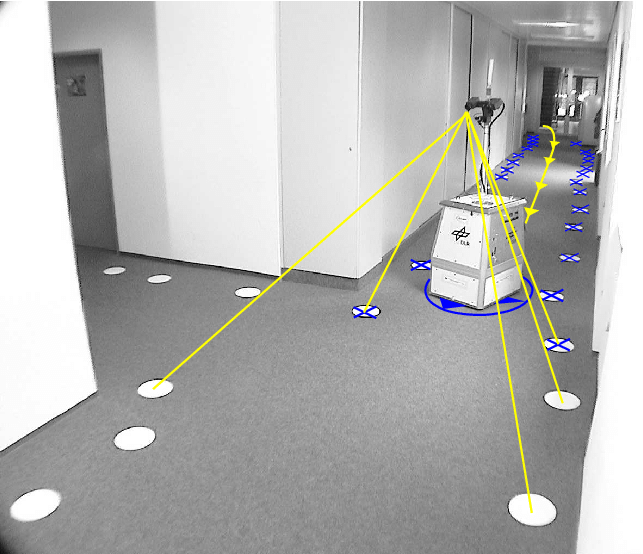
\includegraphics[width=\linewidth]{SLAM_agent} % First image
        \caption[Short caption]{A visual representation of a robot scanning its environment (reproduced from \cite{SLAM_overview})}
        \label{fig:SLAM_agent}
    \end{minipage}\hfill
    \begin{minipage}{0.45\textwidth}
        \centering
        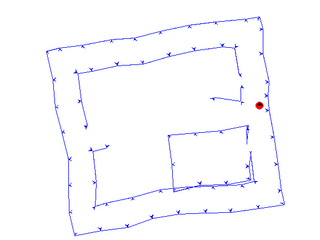
\includegraphics[width=\linewidth]{SLAM_map} % Second image
        \caption[Short caption]{The map (after loop closure) produced by the robot's SLAM algorithm of its environment (reproduced from \cite{SLAM_overview})}
        \label{fig:SLAM_map}
    \end{minipage}
\end{figure}

SLAM (Simultaneous localization and Mapping) is a technique used in robotics to create a map of an unknown environment \cite{SLAM_overview}.
It is an important area of research in robotics as it is heavily used in autonomous vehicles, drones and vacuum cleaners;
allowing agents to understand and navigate their environment effectively. Figure \ref{fig:SLAM_agent} shows an example of a
robot scanning its environment, with the sensors visually added to the image.\\
SLAM can be broken down into two sub-problems: localization and mapping. Localization is the process of determining the
location of a robot in its environment, whilst mapping is the process of constructing a map of the environment. The maps
are constructed using data collected from sensors, such as cameras and laser scanners; Figure \ref{fig:SLAM_map} shows this.
A lot of existing work in SLAM is based on single robot applications, however, there is a growing interest in multi-agent
SLAM.\\
Code implementations of SLAM usually divide the problem into the Front-end and the Back-end \cite{SLAM_components}.
The Front-end is where the agent interprets the environment; it will receive data, which could be in the form of images,
LiDAR scans or other sensor data. The Front-end will then process this data, extracting features and identifying landmarks.
Furthermore, the Front-end will also perform data association, which will compare new features/landmarks to data that has
been previously collected. The Back-end is where the agent will use the data collected from the Front-end to create a map
of the environment and localise itself. There are a number of paradigms which may be used during this process, such as Graph-based
SLAM, Particle filtering and Extended Kalman Filters. By combining the Front-end and the Back-end, the agent will be able to
create an internal representation of its environment and its position in that environment.

\subsection{Background and Evolution of SLAM} % 600 words - currently 513
In the mid 1980s, SLAM concepts were first introduced by Smith and Cheeseman \cite{Early_SLAM}. They initially laid out
the foundations of the problem, which was to be able to reason about the position of an object with potentially inaccurate
information about the environment. Their paper demonstrates a lot of themes which we now associate with SLAM, such as taking
frames (poses) which have an associated positional uncertainty, taking measurements of the environment at each frame and
then using these measurements to identify objects in the environment. Smith and Cheeseman used the Kalman Filter equations
for static-state estimations, and then merged these state estimations to create a representation of the environment.\\
The next major developments in SLAM came shortly after, in the early 90s, from the work of Leonard and Durrant-Whyte.
In their paper, they identify further challenges in SLAM, such as the data association problem and environment dynamics \cite{First_EKF}.
They also outlined one of the traditional problems with SLAM, which is the "chicken and egg" problem. This arises as
to build a useful map, the robot needs to know where it is, and to know where it is, it needs a useful map. To tackle
this, they proposed the use of an Extended Kalman Filter (EKF), which builds on the traditional Kalman Filter equations by
allowing for non-linear state estimations. This was a significant development, as it allowed for the creation of more accurate
maps; however they also concluded that the EKF was not suitable for large-scale environments, as data association becomes
increasingly difficult.\\
Come the 2000s, SLAM had become a well-established area of research, with a number of different paradigms being used to
approach the problem. One of which was FastSLAM, which was developed by Michael Montemerlo and Sebastian Thrun \cite{FastSLAM}.
FastSLAM was an attempt to solve one of the fundamental flaws of EKF SLAM, which was scalability. FastSLAM works by using
a particle filter to estimate the robot's pose, and then constructs a map of the environment using these poses. A particle filter is
a probabalistic technique used to estimate the robots position, which works by having a set of particles randomly distributed
across the environment, which represent possible positions the robot could be in. As the robot moves, the particles are adjusted
based on measurements from the robots sensors; the position of the robot is then estimated by taking the average of the particles.
FastSLAM main strengths are its ability to handle large environments and improve the computational complexity of EFK SLAM, however
it's weaknesses are that it is not as accurate as EKF SLAM and it struggles with dynamic environments.\\

\begin{figure}[h]
    \centering
    \begin{minipage}{0.8\textwidth}
        \centering
        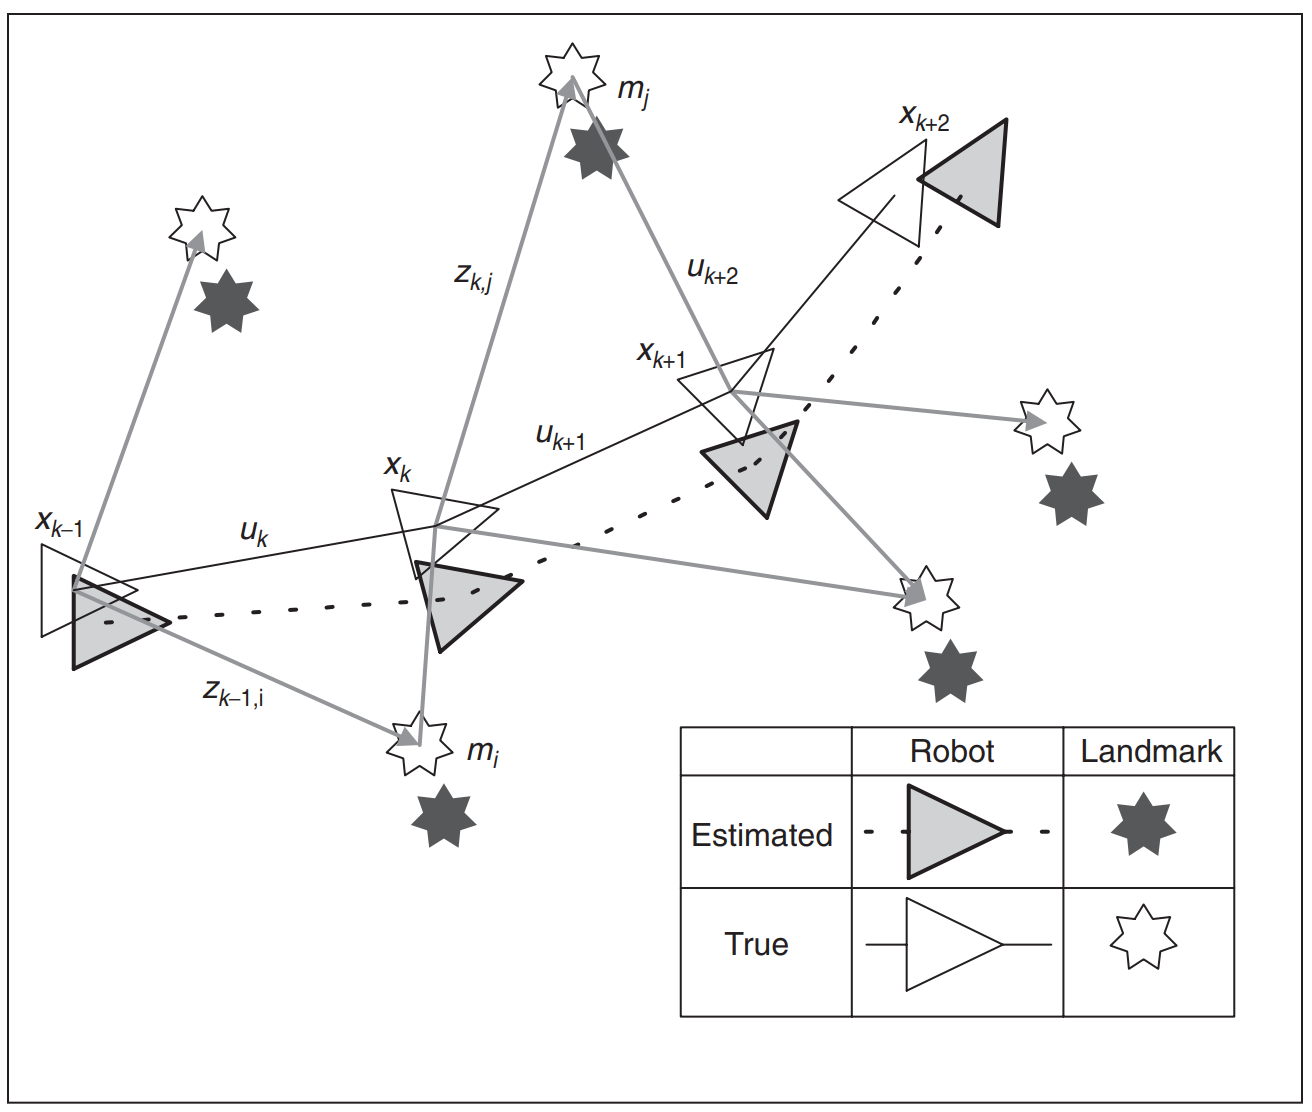
\includegraphics[width=\linewidth]{SLAM_problem} % First image
        \caption[Short caption]{Formal representation of the SLAM problem (reproduced from \cite{SLAM_summary})}
        \label{fig:SLAM_problem}
    \end{minipage}\hfill
\end{figure}

Finally, in 2006 Durrant-Whyte and Bailey wrote a significant paper outlining the future of SLAM \cite{SLAM_summary}. They started by
discussing existing approaches to the problem and then formally outlining the SLAM problem, shown in Figure \ref{fig:SLAM_problem}. They
then went into further detail on how both EFK SLAM and FastSLAM work, and then discussed the limitations of each approach. They also
wrote a second paper, discussing the future of SLAM, including multi-agent SLAM, 3D SLAM and Dynamic environments \cite{Further_SLAM}.

\subsection{Technical Frameworks and Models} % 800 words - currently 1113
\subsubsection{Mapping techniques}
\begin{figure}[h]
    \centering
     \begin{minipage}{0.4\textwidth}
        \centering
        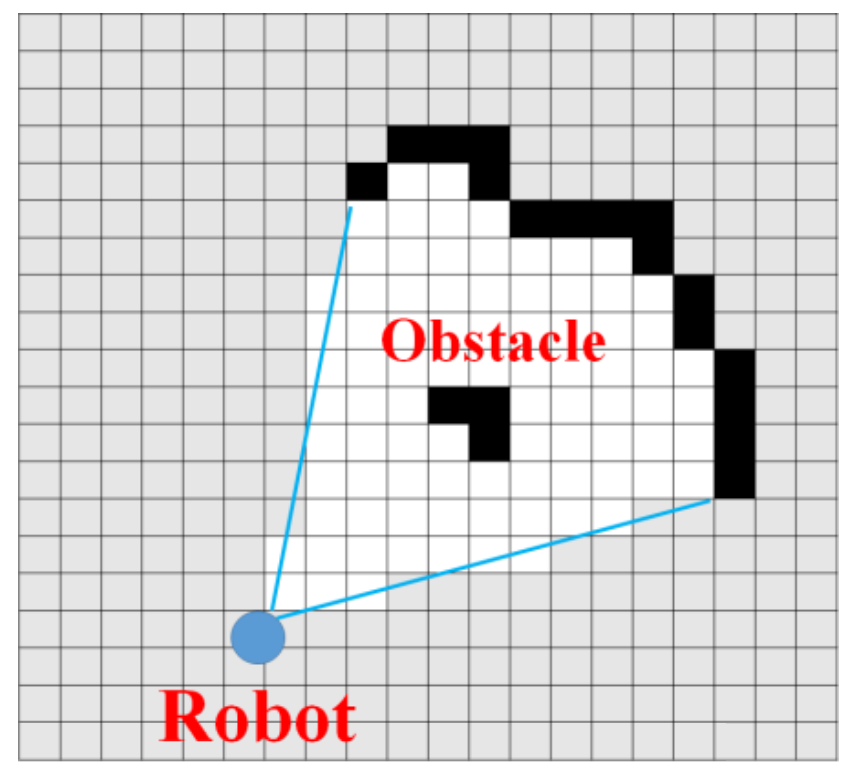
\includegraphics[width=\linewidth]{occupancy_grid} % First image
        \label{fig:simple_occ_grid}
    \end{minipage}\hfill
    \begin{minipage}{0.4\textwidth}
        \centering
        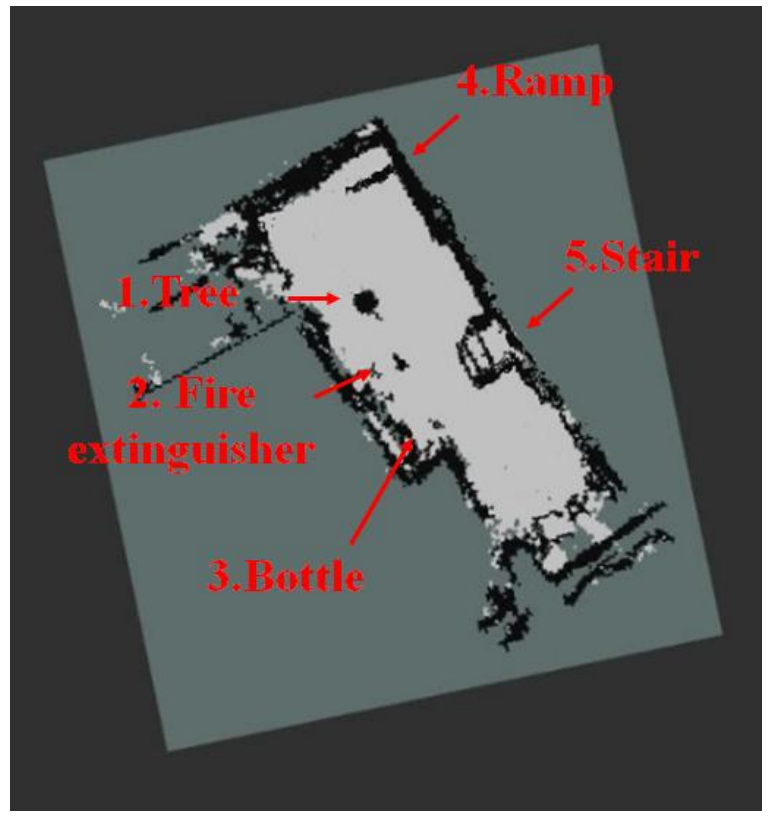
\includegraphics[width=\linewidth]{complex_occ_grid} % Second image
        \label{fig:complex_occ_grid}
    \end{minipage}
    \caption[Short caption]{Example of simple (left) and complex (right) occupancy grids (reproduced from \cite{occupancy_grid})}
\end{figure}

Mapping techniques are used by the agent to create a representation of its environment. There are a number of different mapping techniques
commonly used in SLAM, such as grid maps, feature-based maps and semantic maps. Grid maps, or occupancy maps, are the most common
type of map used in SLAM, as they are easy to implement and computationally efficient. They are typically represented as a 2D array, which
simply stores a binary value for each cell, which represents whether the cell is occupied or not. Figure \ref{fig:simple_occ_grid} shows a simple
example of an occupancy grid, where the black cells represent occupied space and the white cells represent free space. Figure \ref{fig:complex_occ_grid}
demonstrates how an occupancy grid can be used to represent a more complex environment, such as the experiment environment used by Nam
et al \cite{occupancy_grid}. Occupancy grids are typically implemented in conjunction with distance sensors, such as LiDAR - this allows the
agent to measure the distances to multiple points in the environment, which can then be used to update the occupancy grid. \\
Feature-based maps are another common type of map used in SLAM. They work by having the agent detect features in the environment, such as
walls, corners and edges. These features are then used to define landmarks, which are then used to create a map of the environment. Landmarks
are distinct features in the environment which can be used to localise the agent; a common metaphor used to describe landmarks is a distinctive
skyscraper in a city, like the Shard in London, which you could use to figure out your location. Feature-based maps are also implemented with
distance sensors, as the agent can use points detected by the sensor to detect features. \\
\begin{figure}
    \centering
    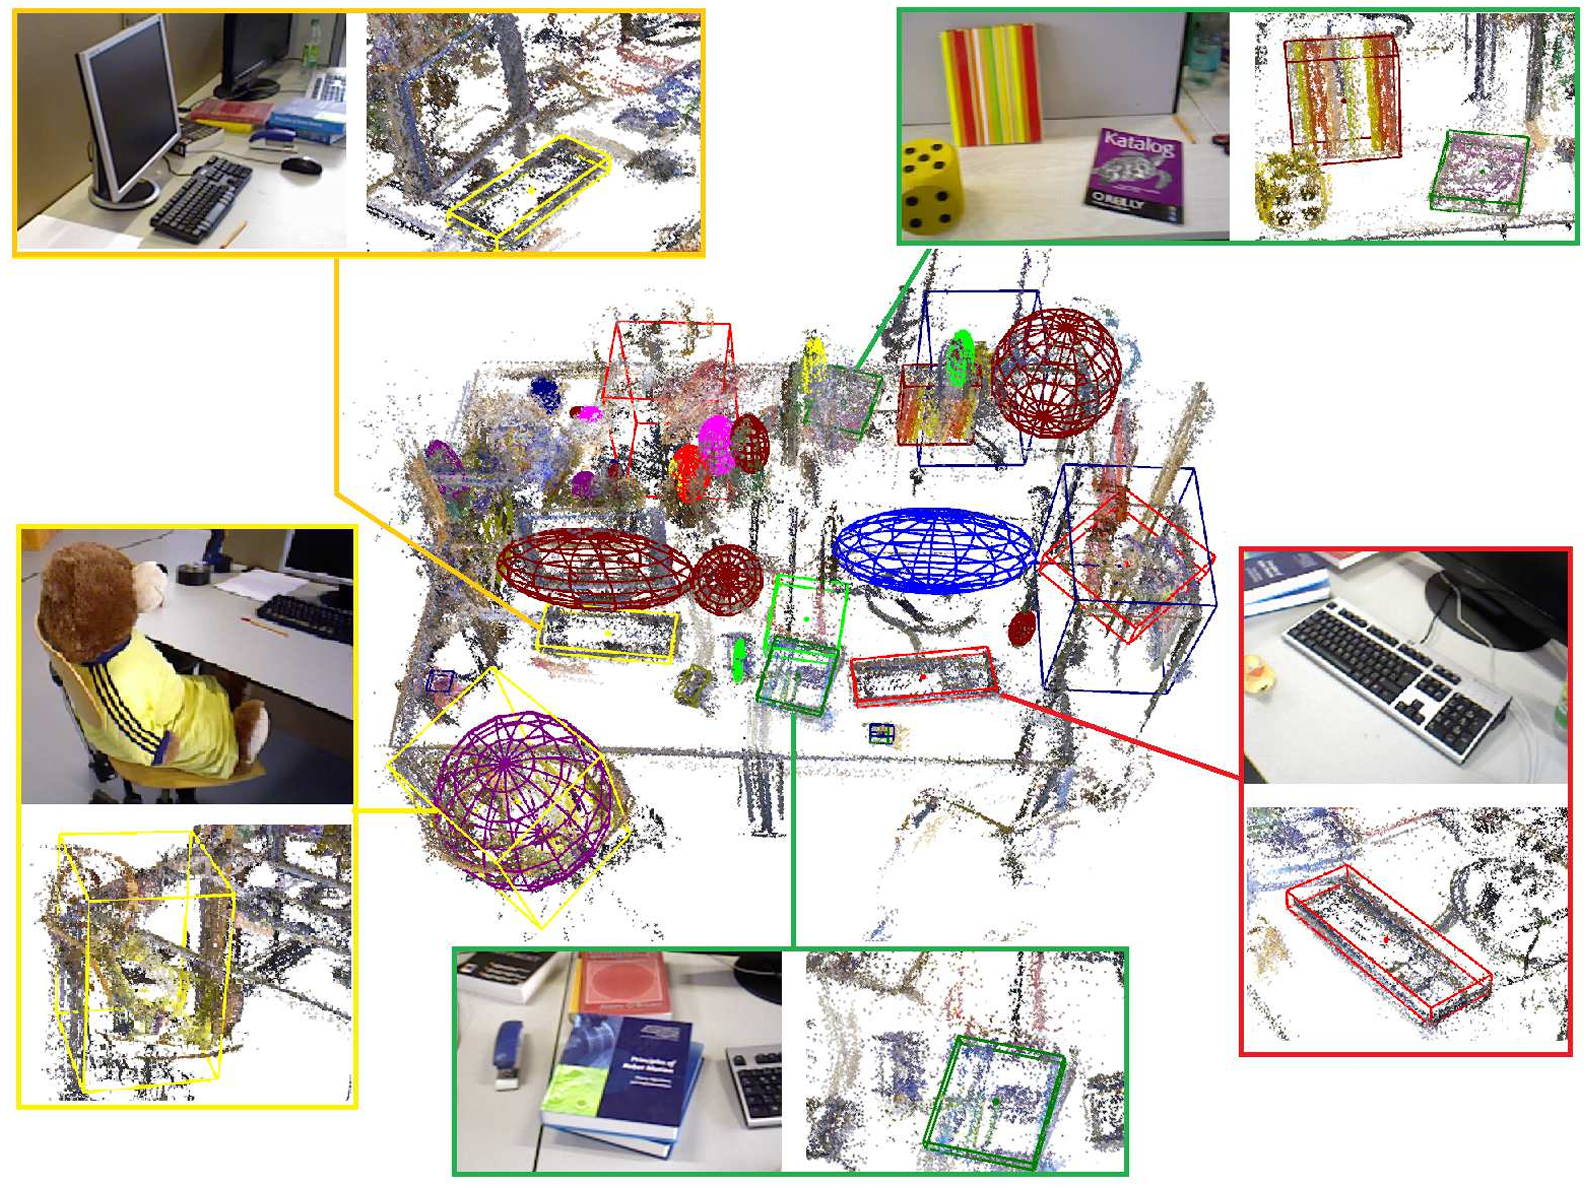
\includegraphics[width=0.7\linewidth]{semantic_maps}
    \caption[Short caption]{Example of a semantic map (reproduced from \cite{semantic_map})}
    \label{fig:semantic_map}
\end{figure}
Finally, semantic maps are a more recent addition to SLAM, which work by allowing the agent to detect and classify objects in the environment.
This is achieved using computer vision techniques, such as object detection and image segmentation. Figure \ref{fig:semantic_map} shows an example
of a semantic map; you can see the image segmentation has identified various objects, such as the keyboard and the books. Semantic maps are used
more frequently in research whilst less often in industry, as they are much more computationally expensive and require more complex sensors, such as
cameras.\\

\subsubsection{Localization techniques}
Localization techniques are used to help the agent determine its position in a given environment. There are a number of popular techniques commonly
used in SLAM, such as Extended Kalman Filters, Particle Filters and Visual Odometry. Extended Kalman Filters are a set of mathematical equations which are used to
estimate the position of the agent given a set of noisy sensor readings. The equations are split into two main functions, the prediction function and the
update function \cite{intro_to_EKF}. The prediction function is used to predict the agents position based on the previous state, which incorporates uncertainty from the
agents movement. The update function is then used to update the agents position based on new sensor readings and update the uncertainty. The prediction functions
are defined as:
\begin{itemize}
    \item State Prediction Equation:
    \begin{equation}
        \hat{x}_{k+1} = f(\hat{x}_{k}, u_{k}, 0)
    \end{equation}
    \item Covariance Prediction Equation:
    \begin{equation}
        P_{k+1} = A_{k} P_{k} A_{k}^T + W_{k} Q_{k} W_{k}^T
    \end{equation}
\end{itemize}
The state prediction equation predicts the next state \(\hat{x}_{k+1}\) based on the previous state \(\hat{x}_{k}\), the control input (the agents desired movement) \(u_{k}\)
and the process noise (which is assumed to be zero here). The covariance prediction equation then updates the uncertainty of the agents position based on the state
transition matrix \(A_{k}\), the previous position uncertainty \(P_{k}\), the control input matrix \(W_{k}\) and the process noise covariance matrix \(Q_{k}\). The update functions are
defined as:
\begin{itemize}
    \item Kalman Gain Equation:
    \begin{equation}
        K_k = P_{k} H_k^T (H_k P_{k} H_k^T + V_k R_k V_k^T)^{-1}
    \end{equation}
    \item State Update Equation:
    \begin{equation}
        \hat{x}_{k} = \hat{x}_{k} + K(z_k - h(\hat{x}_{k}, 0))
    \end{equation}
    \item Covariance Update Equation:
    \begin{equation}
        P_{k} = (I - K_k H_k) P_k
    \end{equation}
\end{itemize}
The Kalman Gain equation determines how impactful the new sensor reading \(z_k\) should be, based on the previous position uncertainty \(P_{k}\). \(H_k\) is the Jacobian of the
measurement function \(h(\hat{x}_{k}, 0)\) with respect to the state, and \(V_k\) is the Jacobian of the measurement function with respect to the measurement noise. The state update
equation then updates the agents position based on the Kalman Gain. Finally, the covariance update equation updates the uncertainty of the agents position based on the Kalman Gain.\\
\begin{figure}[h]
    \centering
     \begin{minipage}{0.24\textwidth}
        \centering
        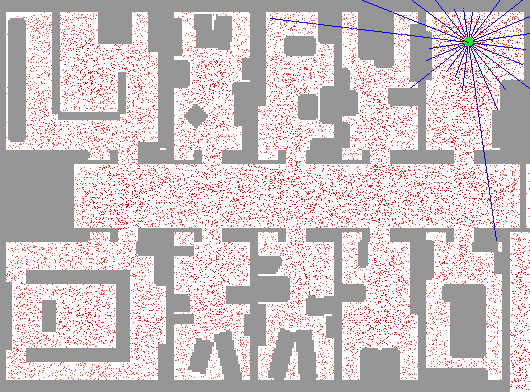
\includegraphics[width=\linewidth]{frame_00_delay-1s} % First image
    \end{minipage}
    \begin{minipage}{0.24\textwidth}
        \centering
        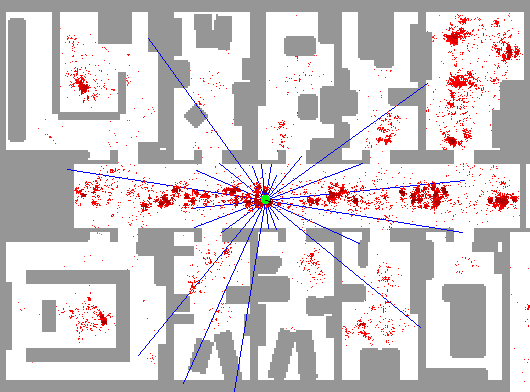
\includegraphics[width=\linewidth]{frame_02_delay-1s}
    \end{minipage}
    \begin{minipage}{0.24\textwidth}
        \centering
        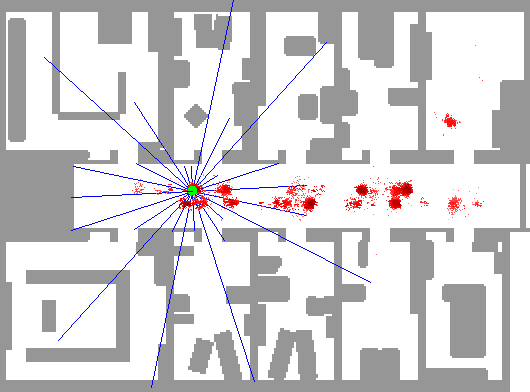
\includegraphics[width=\linewidth]{frame_07_delay-1s}
    \end{minipage}
    \begin{minipage}{0.24\textwidth}
        \centering
        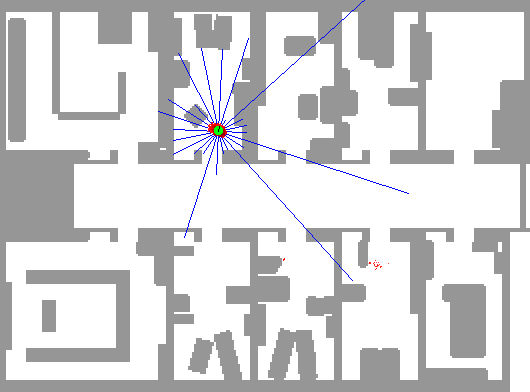
\includegraphics[width=\linewidth]{frame_25_delay-1s}
    \end{minipage}
    \caption[Short caption]{Example of Particle Filter in a 2D environment (reproduced from \cite{particle_filter})}
    \label{fig:particle_filter}
\end{figure}
Particle Filters, or Monte Carlo Localization, is another popular technique used in SLAM, which work by having a set of particles randomly positioned across the environment which represent the
possible positions of the agent (posterior). Each particle is assigned a weight, which represents the probability that the particle's position is the true position of the agent.
As the agent moves, the particles are updated based on sensor readings, which are used to adjust the weights of the particles. The problem can be represented as:
\begin{equation}
    w_i \propto p(z_t | x_i^t)
\end{equation}
Where \(w_i\) is the weight of the particle, \(z_t\) is the observed measurement at time \(t\) and \(x_i^t\) is the state of the particle at time \(t\). As the agent discovers more about its
environment, the particles will converge towards the true position of the agent - as shown in Figure \ref{fig:particle_filter}. Dellaert et al demonstrated the strengths of particle filters in their paper
\cite{monte_carlo_slam}, where they showed that particle filters are able to localise the agent in complex environments, even when the environment is dynamic.\\
Finally, Visual Odometry works by having the agent estimate its position based on visual data. This is achieved using the previously mentioned semantic maps, which are used to detect and classify
objects in the environment. As the name suggests, visual odometry only uses visual data to estimate the agents position; benefits of this approach are that cameras are cheap and lightweight, however
they are also computationally expensive. Furthermore, visual odometry is less effective in environments with poor lighting and textureless surfaces, making it less reliable than other techniques. \\

\subsubsection{Sensor technologies}
There are many different types of sensor technologies used throughout SLAM research, such as LiDAR, cameras and Inertial Measurement
Units (IMUs). LiDAR (Light Detection and Ranging) is a distance sensor which works by shooting out a laser and measuring the time it takes
for the laser to bounce off an object (up to a given distance) and return to the sensor. Typically, the sensor will rotate 360 degrees and take
measurements at regular intervals, which is particularly useful in SLAM as it allows the agent to sense its complete surroundings.\\
Cameras are another common sensor used in SLAM, which work by taking images of the environment and then using computer vision techniques
to extract features and landmarks. One of the advantages of cameras is that they can capture a lot of information about the environment, such
as objects and textures; which make data association easier. However, cameras are also a lot more computationally expensive in comparison to
LiDAR, as feature extraction and landmark detection have a lot more complexity.\\
IMUs are used to measure the orientation, velocity and gravitational forces of the agent; this makes them useful in SLAM as they help record
the agents movement. They are normally used alongside other sensors to help improve the accuracy of the localisation algorithm. \\

\subsection{Algorithms and Implementations} % 700 words - currently 450
\subsubsection{Algorithms}
Graph-based SLAM is a technique used to create a map of an environment, by using a graph to represent the environment. It
works by having a robot move around its environment, whilst taking measurements of its surroundings. These measurements
are usually received by a sensor, such as a camera or laser scanner. The robot then uses these measurements to create a
plot of where objects may be, by combining the measurements from sensors with its memory of the route it has taken. This
technique is used in many applications, both in research and in the real world.\\
One limitation of graph-based SLAM is that it is computationally expensive, as it requires a lot of memory to store the
sensor readings. Also, it is not very scalable, as the more sensors that are added, the more memory is required. Another
limitation is that it cannot always be reliable, as the algorithm depends heavily on detecting loop closures, which when
not detected, can lead to a lot of errors in the map. This, combined with even the slightest inaccuracy from sensors/motors
makes it difficult to apply to the real world.\\
Oriented FAST and Rotated BRIEF (ORB) SLAM is a real-time, visual SLAM algorithm which works by using a camera to detect features
in the environment. A real-time SLAM algorithm is one that can process data as it is received - this is significant for ORB SLAM
as the camera input is very computationally expensive to analyse. ORB SLAM works by detecting features in the environment, such
as corners and edges, and then using these features to create a map of the environment; typically done using the previously
mentioned semantic maps. Originally, ORB SLAM was a development of bundle adjustment, which is a technique used to get accurate
estimations of the agents positions, but isn't real-time \cite{ORB_SLAM}. A popular use case of ORB SLAM is in autonomous vehicles,
as modern vehicles are equipped with cameras and powerful computers, which can be used to run complex algorithms.\\
Hector SLAM is a more recent development in SLAM, which uses LiDAR to create a map of the environment. It is significant because it
differs from other previously mentioned techniques by relying less on wheel odometry and other forms of motion estimation. Instead,
Hector SLAM employs a scan matching algorithm, which works by comparing the current LiDAR scan to previous scans, and using the
differences to estimate the agents position. Hess et al implemented Hector SLAM using a branch and bound algorithm, which allowed
them to find the best match between scans \cite{Hector_SLAM}; other implementations have used gradient descent to achieve similar
results. Overall, this technique is particularly useful in environments where wheel information is less reliable, such as on rough terrain
or on slippery surfaces. \\

\subsubsection{Software}
There are a number of existing tools and packages that can be used to implement and simulate SLAM algorithms; including Robot Operating System (ROS),
Mobile Robot Programming Toolkit (MRPT), Webots, Enki, Gazebo and CoppeliaSim (formally V-REP). The mentioned resources can be split into
two distinct groups: algorithm implementations and simulation environments. Packages like ROS and MRPT fall under the former, providing tried
and tested SLAM algorithms. ROS is an open-source package which was created using C++ and Python, and is now widely used in both research
and industry. More recently, development of ROS2 has picked up pace, which is a more modern version of ROS, aiming to be more appropriate
for modern applications. MRPT offers a number of SLAM algorithms which can be used in both 2D and 3D environments, and as the name suggests,
is particularly useful for mobile robots.\\
Enki, Gazebo and Webots are all robot simulator packages, which contain a number of premade robots and environments. They are particularly
useful for testing SLAM algorithms, as it allows the user to create custom environments and test the algorithms in a controlled and realistic
setting. Enki is written in C++ and is open-source, which makes it easy to modify and extend. Gazebo can be used to create 3D environments,
which can be used to test visual SLAM algorithms. Webots also allows for modelling, programming and simulating robots in 3D environments;
the package is widely used in research and education. All of these packages are typically used in conjunction with packages that implement
SLAM algorithms, like ROS.\\



\subsection{Real-world Applications and Case Studies} % 600 words - currently 196
SLAM has a number of real-world applications, such as autonomous vehicles, drones, vacuum cleaners and search and rescue.
In the context of drones, UAV (Unmanned Aerial Vehicles) SLAM is used to help drones navigate their environment. This is
particularly challenging as drones are often used in dynamic environments. Furthermore, drones often operate at fast speeds,
which means the SLAM algorithm needs to be able to process data quickly. UAV SLAM can be implemented using similar techniques
to ground-based SLAM, using LiDAR and cameras for feature detection; Caballero et al demonstrated how visual SLAM can be used
in this context \cite{UAV_SLAM}.\\
Another application of SLAM is in Virtual Reality (VR) and Augmented Reality (AR) technologies. SLAM is used in VR and AR to
help localise the headset in the environment, which is important for creating realistic and consistent movement. Kuo et al
demonstrated this well in their paper, where they used ORB SLAM 2 to localise a VR headset in a 3D \cite{VR_SLAM}. Their
implementation involved using a VR headset to control a robot; they were able to demonstrate that the error rate of the SLAM
algorithm was at least 0.5cm, which is accurate enough for most VR applications.\\

\newpage

\section{Requirements Analysis}
Table~\ref{tab:requirements_table} shows the requirements for my project, along with their justification. Initially, I will
create a simulation interface, where the user can see the agents and the environment. After, I will work towards implementing
core parts of the SLAM algorithm, such as feature extraction and landmark detection. I will then attempt to implement a Kalman
Filter, which the agent will use to localise itself in the environment. Finally, I will work towards adding data association, which will
hopefully complete the SLAM algorithm. The latter stages of the project will be spent on evaluating the performance of the algorithm
and documenting my findings. I have also added a couple optional requirements, which can be carried out should time permit but are
not critical towards the success of the project.\\
When creating the simulation interface, I will be using the Python programming language, along with the PyGame library. This
will abstract away a lot of the complexity of creating a graphical user interface, allowing me to focus on the core functionality.
I have chosen to use Python in my project as it is a language I am familiar with and is widely documented, which will be useful
should I run into issues. I will also use various other scientific python libraries throughout my project, such as NumPy, SciPy and
Matplotlib.\\
 I have chosen to create my own simulation environment, instead of using an existing package, as I believe this will give me more
control over the project. I enjoy knowing how each component of my project works, and by creating my own environment, I will be able
to create a more tailored solution.\\
\begin{table}[H]
    \centering
    \begin{tabular}{|p{0.03\linewidth}|p{0.17\linewidth}|p{0.17\linewidth}|p{0.53\linewidth}|}
        \hline
        \textbf{ID} &
        \textbf{Requirement Type} &
        \textbf{Requirement} &
        \textbf{Justification}\\
        \hline
        \textbf{1} &
        Funcitonal &
        Simulation Interface &
        A graphical user interface will be critical for demonstrating the agents behaviours, and will also aid de-bugging. Pygame
        will make it easy to watch the algorithm in real-time and visualise the mapping process.\\
        \hline
        \textbf{2} &
        Funcitonal &
        Implement the Extended Kalman Filter (EFK) algorithm &
        EFK will be essential for estimating the state of the agent and the uncertainty related to it's position, and the position
        of other agents.\\
        \hline
        \textbf{3} &
        Funcitonal &
        Simulation Environment Creation &
        In order for SLAM to work, a simulated environment will be needed. This will help me demonstrate the SLAM algorithm and
        test its performance. \\
        \hline
        \textbf{4} &
        Non-Funcitonal &
        Program Performance &
        The program will need to be efficient and the UI should be smooth. This is necessary to help provide a realistic demonstration
        of the SLAM algorithm.\\
        \hline
        \textbf{5} &
        Non-Funcitonal &
        Modularity &
        The program should be modular, allowing for easy changes to both the agents behaviour and the environment. This is important
        as it will allow me to easily test different scenarios and variations of the SLAM algorithm.\\
        \hline
        \textbf{6} &
        Non-Funcitonal &
        Documentation and Code Comments &
        The code should be well documented and commented, as this will help make the codebase more maintainable and easier to
        understand.\\
        \hline
    \end{tabular}
    \caption{Table of requirements and their justification}\label{tab:requirements_table}
\end{table}\\

Along with this table of requirements, there will also be a number of opportunities for optional extensions, should time permit.
These include:
\begin{itemize}
    \item Implementing physical robots.
    \item User interface enhancements, such as adding being able to view each individual agents internal map.
    \item Implementing a more complex SLAM algorithm, such as FastSLAM.
\end{itemize}

\section{Project Plan}
\begin{figure}[H]
    \centering
    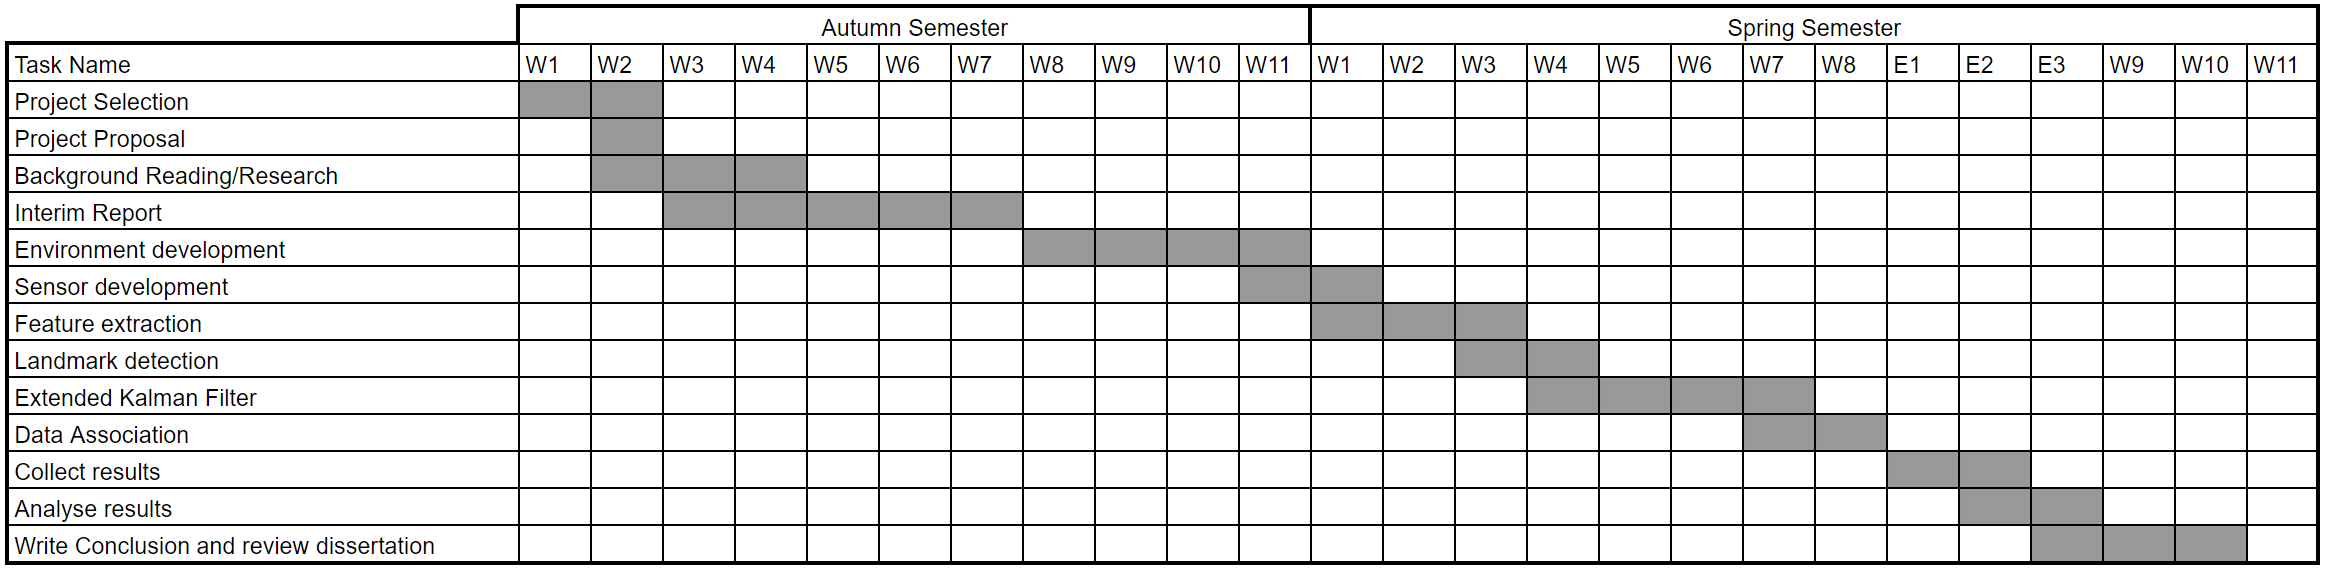
\includegraphics[width=0.8\linewidth]{gantt_chart.png}
    \caption{Gantt chart showing the project plan}
    \label{fig:gantt_chart}
\end{figure}
The execution of my project will be split into various phases, where each phase will focus on an area of development.
In order to remain focused, I will be using an agile-like approach, where I will be working in short sprints to complete
certain tasks, then writing and reflecting on them in my report. Figure \ref{fig:gantt_chart} shows the project plan,
where the grey bars represent the time spent at each phase. Should my project overrun, I will have contingency time
built into both the Christmas break and prior to the due date, which is currently unaccounted for in the project plan.
I have also tried to be realistic with my time estimations, allowing for a reasonable amount of time to complete each
phase.\\

\subsection{Phase 1 - Research and Planning}
The first phase of my project involves researching and planning. During this period I will create a project proposal,
research single and multi-agent SLAM algorithms, and write my interim report. This phase will be completed by week 7. It is
important to carry out this phase as it provides structure for the whole project, which will help ensure that the project is
completed on time.

\subsection{Phase 2 - Project Setup}
The second phase of my project will be to develop the simulation environment and sensors for the agent. This will involve
creating a graphical user interface, using the PyGame library, where the user can see the agent, the environment and a
representation of the agents internal map. I will then create a sensor which can detect the presence of walls and objects
in the environment. I plan on implementing a LiDAR sensor, as this will provide my feature detection system with the information
it should require. This phase will be completed by week 11 - putting me in a good place to work on implementing SLAM algorithm
after the Christmas break.

\subsection{Phase 3 - Data Preprocessing}
The third phase of my project will be to establish the fundamenals of the SLAM algorithm. I will start by implementing a feature
extraction system, which will be used to draw lines and edges through points detected by the LiDAR sensor. I will then work on
identifying landmarks, which will be used to create a map of the environment. After implementing these, I will spend some time
writing up my methods in my report, ensuring that I have a clear understanding of the algorithms I have implemented. This phase
should be completed by week 4 of the Spring semester.

\subsection{Phase 4 - Algorithm Implementation}
The fourth phase of my project will be to implement the core parts of the SLAM algorithm. I will start by implementing a Extended
Kalman Filter, which will be used to estimate the agents position and the position of landmarks in the environment. I will then
implement a data association algorithm, which will be used to compare new features to existing landmarks. After completing this
work, I should have fully implemented the SLAM algorithm. I expect this stage of the implementation to take the longest, so I have
allocated a significant amount of time to complete it. This phase should be completed by week 8 of the Spring semester.

\subsection{Phase 5 - Analysis and Conclusion}
I will start the final phase of my project during the Easter break, where I will collect data which will be used to analyse
the performance of the algorithm. I will then use this data to create a series of graphs and charts, which will be used to
visualise performance and draw conclusions. After, a lot of time will be spent writing up my findings and analysing the performance
of the algorithms. Finally, I will finish my project by writing a conclusion, which will summarise my findings and discuss
potential future work. Prior to submitting my report, I will also spend time proofreading and editing my work.

\section{Professional and Ethical Considerations}
My project maintains compliance towards all ethical considerations, as there is minimal external involvement from
humans. The majority of my project will be carried out in simulation, therefore no ethical approval is required. Should
my project progress to physically implementing agents, considerations such as safety around the robots, will be considered.
All tests will be carried out in an environment where people cannot be hit, therefore mitigating any trip hazards.\\

To ensure all elements of the BCS code of conduct are met, I have summarised each section and how I meet certain criteria. \\
\subsection{Public Interest}
As mentioned previously, my project has due regard for public health, as there is minimal external involvement from humans.
Furthermore, no major privacy, security or wellbeing considerations are required due to the nature of this project. Third parties
will be respected throughout the project with consistent citations and there will be no discrimination against anybody involved.
Finally, I will promote equal access to the benefits of IT by open-sourcing my research once I have graduated. This will be accessible
on my Github profile: \href{https://github.com/CharlieAnthony/}{https://github.com/CharlieAnthony/} \\
\subsection{Professional Competence and Integrity}
My project is within my professional competence, as it significantly relies upon knowledge obtained from modules such as "Acquired
Intelligence and Adaptive Behaviour" and "Fundamentals of Machine Learning." Furthermore, I will develop my professional knowledge,
skills and competence through communicating with my supervisor and ensuring all relevant gaps in knowledge are explored through
reading extensively. As part of my background reading, I have made myself familiar with the BCS code of conduct and surrounding
legistlation. I will comply with this throughout when carrying out my professional responsibilities. There will also
be no unethical inducements offered or accepted throughout the project. \\
\subsection{Duty to Relevant Authority}
As the relevant authority will be the University of Sussex, I will comply with all relevant codes of conduct and legislation. I
will exercise my professional judgement at all times, including avoidance of any situation that may give rise to a conflict of
interest between myself and the university. I will also make it my responsibility to ensure all colleagues work is properly
referenced in a bibliography at the end of my dissertation. \\
\subsection{Duty to the Profession}
Finally, I accept my duty to uphold the reputation of the profession. I will work to the best of my ability to ensure my project
is complete to the highest possible standard. As mentioned previously, I will seek to improve professional standards through
communication with my supervisor. This dissertation will be written with integrity and respect towards all members of BCS and colleagues
of the profession. \\


%Related Work

\section{Methods}

\subsection{Random Walk Exploration}
To be able to create a map of the environment, the agent must first explore the environment. One of the simplest exploration strategies
is random walk exploration, where the agent moves in a random direction until it hits an obstacle. This is a common strategy used in
SLAM, as it is easy to implement and computationally efficient; however it is by no means the best strategy for exploration. \\
\begin{algorithm}
    \caption{Random Walk Exploration Algorithm}\label{alg:random_walk}
\begin{algorithmic}
    \State $reading \gets get\_sensor\_reading()$
\end{algorithmic}
\end{algorithm}

\subsection{Feature Extraction}
Feature extraction is the process of detecting and extracting features from sensor data. In the context of SLAM, features
are points of interest in the environment, such as corners, edges and lines. These features can then be used to create a map
of the environment. There are many different techniques for feature extraction, such as the Harris corner detector and the
split-and-merge algorithm. My implementation uses Seeded region growing, which was proposed by Gao et al.
\cite{seeded_region_growing}.\\
Seed segment detection works by observing a set of points from a single sweep. The algorithm starts by fitting a line through
the given points. Then, in order for a seed segment to be further considered, it must satisfy the following two conditions:
\begin{itemize}
    \item The distance between the point and the line must be less than a given threshold.
    \item The distance between the point and it's predicted position must be less than a given threshold.
\end{itemize}
Seed segment detection uses orthogonal line fitting to propose a feature through a set of points, as it is more effective
than using traditional methods, such as standard least square fitting; this is due to the nature of least square fitting
which only takes into account the vertical distances of each point.\\
After, the algorithm applies region growing, which helps create line segments; which will then become our features. The
region growing works by examining neighbouring points and adding them to the line segment if they satisfy the same conditions.
This process is repeated until no more points can be added to the line segment.\\

\subsection{Identifying Landmarks}

\subsection{Extended Kalman Filter}

\subsection{Data Association}




    \section{Appendices}

\subsection{Supervisor Meetings}    % 720 words

\subsubsection{Meeting 1 - 11/10/2023}
Discussed on the project idea and potential directions to take. Discussed the possibility of implementing physical agents,
challenges that may occur and potential ways of implementing swarm algorithms. Need to focus on researching SLAM and swarm
and looking into existing resources.
\subsubsection{Meeting 2 - 27/10/2023}
Discussed potential algorithms, such as particle filters and graph-based SLAM. We also discussed the logistics of the project,
ensuring that it remains both realistic and achievable. We also discussed the possibility of implementing physical agents,
and where relevant resources could be found.
\subsubsection{Meeting 3 - 14/11/2023}
Started with feedback on the interim report - discussing the structure and content. After we discussed how the project will
move forward and the next steps to take. Given the interim report is now complete, we can focus mainly on development, following
the project plan. As I have already developed a basic simulation interface, I can now move onto implementing my first SLAM algorithm.
\subsubsection{Meeting 4 - 08/12/2023}
In this meeting, we turned to ironing out the specifics of the implementation - including looking at existing resources, like
Enki, and concepts that need to be considered, such as Differential Turning. The goal of this meeting was to guide me into
starting to create my environment and first SLAM algorithm, which will be implemented over the christmas break.
\subsubsection{Meeting 5 - 02/02/2024}
We firstly caught up on progress made over the christmas break. After, we started to look forward to the next steps of the project,
discussing the projects overall direction and the next steps to take. One notable suggestion was the move away from swarm algorithms
and perhaps the move towards multi-agent SLAM, as this would be more achievable in the time frame. Finally, we discussed how I
should manage my time towards the end of the project and how I could start working on my dissertation.
\subsubsection{Meeting 6 - 09/02/2024}
Started with me demonstrating my current progress, with my environment working, LIDAR sensor appropriately implemented and
my work-in-progress feature detection. We discussed then how I could approach landmark detection and how I planned on implementing
it. We ended the meeting with clearing up questions regarding the project presentation, poster competition and submission.
\subsubsection{Meeting 7 - 16/02/2024}
We discussed how my project was going; talking about feature extraction and landmark detection. As I had been having troubles
with bugs in the previous week, Chris suggested spending more time writing test cases. We then discussed how I should approach
writing the final report; considering structure and content. We agreed that there are parts of the report that I could start
now, such as my literature review and methodology used in feature detection and landmark detection.
\subsubsection{Meeting 8 - 23/02/2024}
Started with showing my progress on landmark detection and randon walk exploration. We then discussed different exploration
algorithms that could be used, as random walk exploration isn't efficient. We discussed creating some form of wall-avoidance
navigation, which would be far more efficient. We then reviewed my plan and reflected on how progress was going. We both
agreed that progress isn't as fast as we would like, but we are still on track to complete the project on time.
\subsubsection{Meeting 9 - 29/02/2024}
We had a quick online meeting this week; discussing where the project is and the next steps. We started by talking about
my implementations of exploration strategies and how I could improve them. We then discussed evaluation metrics and how I
could gather and present data. Finally, we talked about how I could approach multi-agent SLAM, as it's an area I am concerned
about due to it's complexity.
\subsubsection{Meeting 10 - 15/03/2024}
This meeting was a clear turning point in the project. As progress hadn't proceeded as expected, we discussed the scope of
the project and how it could be adjusted to ensure that I could complete it on time. We agreed that I should focus on the single-agent
components of SLAM, as they are the most important parts of my project. We also discussed how I could approach the final report -
including changes that would need to be made to adhere to the new project scope. Finally, we discussed in further detail how I could
gather data for my analysis and how I could present it.
\subsubsection{Meeting 11 - 22/03/2024}
As the final decisions had been made, a lot of the previous week was spent working on my paper; therefore there wasn't much to show.
We met on zoom and discussed the rate of progress, how the report is coming along and suggestions about my referencing. We also
discussed the presentation some more, as it has been an area troubling me. Chris talked me through the process - stating that it should
just be a summary of my project, really focusing on the key points and results. This was the last meeting before the easter break, so
progress should increase after this point.
\subsubsection{Meeting 12 - 03/04/2024}
We met during the easter break on zoom to catch up about on progress. Chris provided some general feedback on the earlier sections
of my paper, suggesting how I could adjust it's content to create a more balanced report. We then talked about how the code was
coming along; I talked through some of the troubles I've had with the EKF implementation and Chris made some suggestions about
how I could approach it differently. We finished by talking through my plan for the final weeks of the project - I discussed a rough
plan I had constructed and Chris confirmed that it seemed appropriate.


\subsection{Project Proposal}
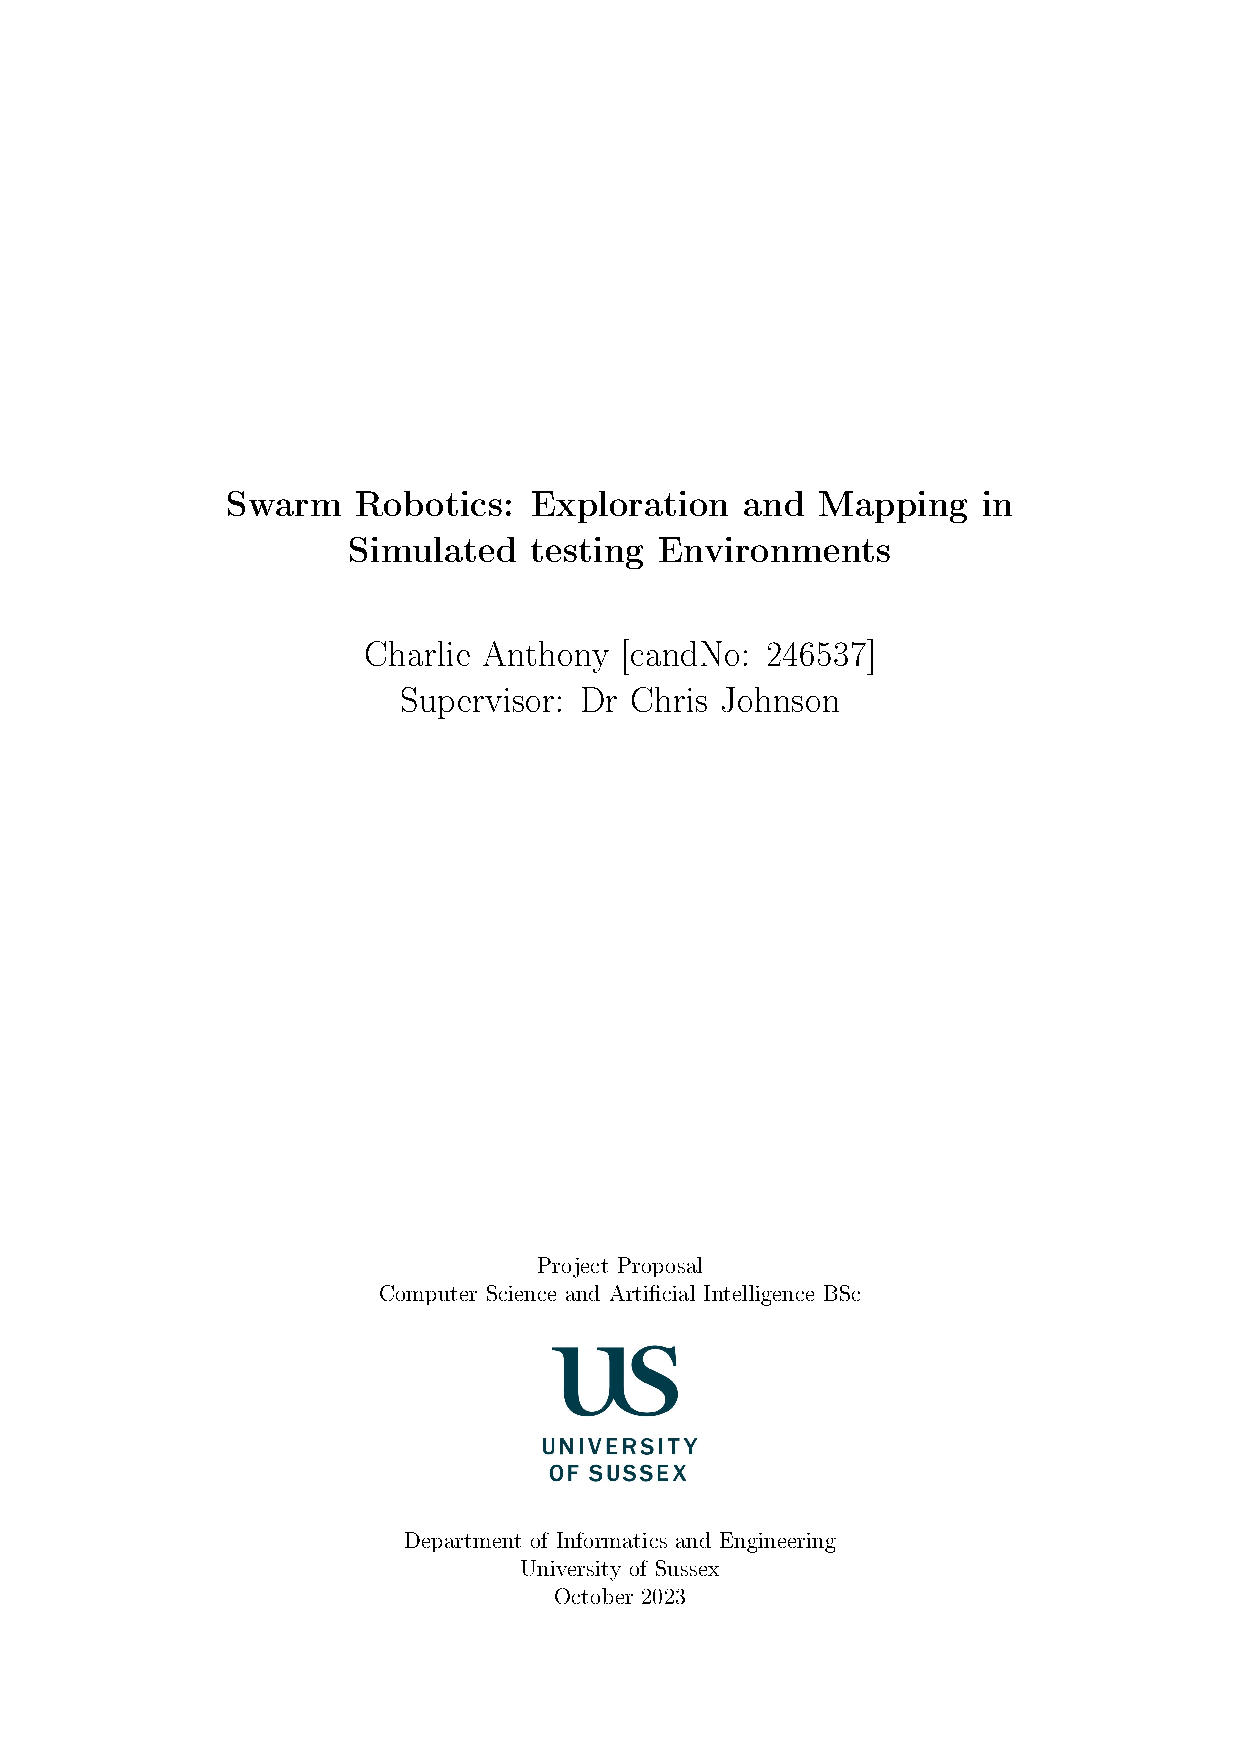
\includepdf[pages=-]{ProjectProposal.pdf}

%References

\section{References}

\begin{thebibliography}{9}

    \bibitem{SLAM_overview}
    Frese, U., Wagner, R. and Röfer, T. (2010). A SLAM Overview from a User’s Perspective.
    \textit{KI - Künstliche Intelligenz}, 24(3), pp.191–198.
    \href{http://dx.doi.org/10.1007/s13218-010-0040-4}{http://dx.doi.org/10.1007/s13218-010-0040-4}

    \bibitem{SLAM_components}
    Alsadik, B. and Karam, S. (2021) The Simultaneous Localization and Mapping (SLAM)-An Overview.
    \textit{Journal of Applied Science and Technology Trends, 2(02), pp. 147 - 158.}
    \href{https://doi.org/10.38094/jastt204117}{https://doi.org/10.38094/jastt204117}

    \bibitem{Early_SLAM}
    Smith, R.C.; Cheeseman, P. (1986). "On the Representation and Estimation of Spatial Uncertainty".
    \textit{The International Journal of Robotics Research. 5 (4): 56–68.}
    \href{https://doi.org/10.1177/027836498600500404}{https://doi.org/10.1177/027836498600500404}

    \bibitem{First_EKF}
    J. J. Leonard and H. F. Durrant-Whyte, "Simultaneous map building and localization for an autonomous mobile robot,"
    \textit{Proceedings IROS '91:IEEE/RSJ International Workshop on Intelligent Robots and Systems '91, Osaka, Japan, 1991, pp. 1442-1447 vol.3,}
    \href{https://doi.org/10.1109/IROS.1991.174711}{https://doi.org/10.1109/IROS.1991.174711}

    \bibitem{FastSLAM}
    Montemerlo, M., Thrun, S., Koller, D. and Wegbreit, B., 2002. "FastSLAM: A factored solution to the simultaneous localization and mapping problem,"
    \textit{Proceedings of the AAAI National Conference on Artificial Intelligence. pp. 593-598}.

    \bibitem{SLAM_summary}
    Durrant-Whyte, H. and Bailey, T. (2006). "Simultaneous localization and mapping: part I",
    \textit{IEEE Robotics & Automation Magazine, [online] 13(2), pp.99–110}.
    \href{https://doi.org/10.1109/mra.2006.1638022}{https://doi.org/10.1109/mra.2006.1638022}

    \bibitem{Further_SLAM}
    T. Bailey and H. Durrant-Whyte, "Simultaneous localization and mapping (SLAM): part II,"
    \textit{IEEE Robotics & Automation Magazine, vol. 13, no. 3, pp. 108-117, Sept. 2006}.
    \href{https://doi.org/10.1109/MRA.2006.1678144}{https://doi.org/10.1109/MRA.2006.1678144}

    \bibitem{occupancy_grid}
    Nam, Tae & Shim, Jae & Cho, Young. (2017). "A 2.5D Map-Based Mobile Robot Localization via Cooperation of Aerial and Ground Robots",
    \textit{Sensors 17(12): 2730}.
    \href{http://dx.doi.org/10.3390/s17122730}{http://dx.doi.org/10.3390/s17122730}

    \bibitem{semantic_map}
    Y. Wu, Y. Zhang, D. Zhu, Y. Feng, S. Coleman and D. Kerr, (2020). "EAO-SLAM: Monocular Semi-Dense Object SLAM Based on Ensemble Data Association,"
    \textit{IEEE/RSJ International Conference on Intelligent Robots and Systems (IROS), pp. 4966-4973},
    \href{https://doi.org/10.1109/IROS45743.2020.9341757}{https://doi.org/10.1109/IROS45743.2020.9341757}

    \bibitem{intro_to_EKF}
    Welch, G. and Bishop, G. (1995). An Introduction to the Kalman Filter.
    \textit{online}
    Available at: \href{https://perso.crans.org/club-krobot/doc/kalman.pdf}{https://perso.crans.org/club-krobot/doc/kalman.pdf} (Accessed: 13 February 2024)

    \bibitem{particle_filter}
    Kim, S. (2023). "FastSLAM: Algorithm for Simultaneous Localization and Mapping,"
    \textit{[online] MLPurdue.}
    Available at: \href{https://medium.com/ml-purdue/fastslam-algorithm-for-simultaneous-localization-and-mapping-6fb5bd141f30}{https://medium.com/ml-purdue/fastslam-algorithm-for-simultaneous-localization-and-mapping-6fb5bd141f30}. (Accessed: 20 March 2024)

    \bibitem{monte_carlo_slam}
    F. Dellaert, D. Fox, W. Burgard and S. Thrun, (1999). "Monte Carlo localization for mobile robots,"
    \textit{Proceedings 1999 IEEE International Conference on Robotics and Automation (Cat. No.99CH36288C), pp. 1322-1328 vol.2,}
    \href{https://doi.org/10.1109/ROBOT.1999.772544}{https://doi.org/10.1109/ROBOT.1999.772544}

    \bibitem{ORB_SLAM}
    R. Mur-Artal, J. M. M. Montiel and J. D. Tardós, (2015). "ORB-SLAM: A Versatile and Accurate Monocular SLAM System,"
    \textit{IEEE Transactions on Robotics, vol. 31, no. 5, pp. 1147-1163,}
    \href{https://doi.org/10.1109/TRO.2015.2463671}{https://doi.org/10.1109/TRO.2015.2463671}

    \bibitem{Hector_SLAM}
    W. Hess, D. Kohler, H. Rapp and D. Andor (2016). "Real-time loop closure in 2D LIDAR SLAM,"
    \textit{2016 IEEE International Conference on Robotics and Automation (ICRA), pp. 1271-1278,}
    \href{https://doi.org/10.1109/ICRA.2016.7487258}{https://doi.org/10.1109/ICRA.2016.7487258}

    \bibitem{VR_SLAM}
    Chen-Yu Kuo, Chun-Chi Huang, Chih-Hsuan Tsai, Yun-Shuo Shi, Shana Smith, (2021). "Development of an immersive SLAM-based VR system for teleoperation of a mobile manipulator in an unknown environment,"
    \textit{2021 Computers in Industry, Volume 132, 103502, ISSN 0166-3615,}
    \href{https://doi.org/10.1016/j.compind.2021.103502}{https://doi.org/10.1016/j.compind.2021.103502}

    \bibitem{UAV_SLAM}
    Caballero, F., Merino, L., Ferruz, J. et al. "Vision-Based Odometry and SLAM for Medium and High Altitude Flying UAVs,"
    \textit{J Intell Robot Syst 54, 137–161 (2009),}
    \href{https://doi.org/10.1007/s10846-008-9257-y}{https://doi.org/10.1007/s10846-008-9257-y}

    \bibitem{seeded_region_growing}
    Gao, H., Zhang, X., Fang, Y. and Yuan, J. (2018). A line segment extraction algorithm using laser data based on seeded region growing.
    \textit{ International Journal of Advanced Robotic Systems}, p.172988141875524.
    \href{https://doi.org/10.1177/1729881418755245}{https://doi.org/10.1177/1729881418755245}

\end{thebibliography}



\end{document}


